\chapter{Generación de una aplicación con JHipster}
\label{anex:2}

\drop{E}{ste} anexo será una guía que explicará cómo generar con JHipster una aplicación de características similares a ONCOSUP. Aunque no se exploren, se podrán ver las diferentes opciones de generación que ofrece la herramienta.

Antes de comenzar la generación de la aplicación es necesario poner a punto en entorno de trabajo. Se comenzará por ir a la web de Oracle y comprobar que la versión de java instalada es la 8 o superior (\url{http://www.oracle.com/technetwork/java/javase/downloads/index.html}).

A continuación, se debe acceder al sitio de \emph{Node.js} y descargar la última versión estable (\url{https://nodejs.org/en/}). No es necesario cambiar nada en la configuración de instalación.

Es necesario instalar \emph{Yarn}, un gestor de dependencias (\url{https://yarnpkg.com/en/docs/install#windows-stable}).

Finalmente, se debe abrir una consola de comandos para poder realizar la instalación de JHipster con el comando: \texttt{\$ yarn global add generator-jhipster}.

Con estos pasos previos el entorno está listo para generar la primera aplicación con JHipster. Para ello, en una consola de comandos, se crea la carpeta en la que se desea generar la aplicación y se accede a ella (figura \ref{fig:1}).

\begin{figure}[!h]
\begin{center}
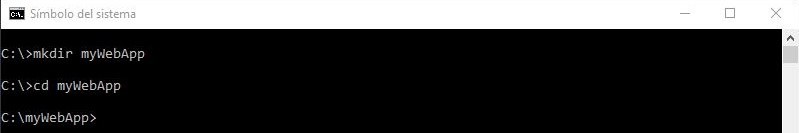
\includegraphics[width=1\textwidth]{1}
\caption{Creación de la carpeta para el proyecto}
\label{fig:1}
\end{center}
\end{figure} 
\clearpage
Una vez se está ubicado en la carpeta en la que se desea generar la aplicación, se ejecuta el comando: \texttt{\$ jhipster}. Se podrá ver como se inicia la generación (figura \ref{fig:2}).

\begin{figure}[!h]
\begin{center}
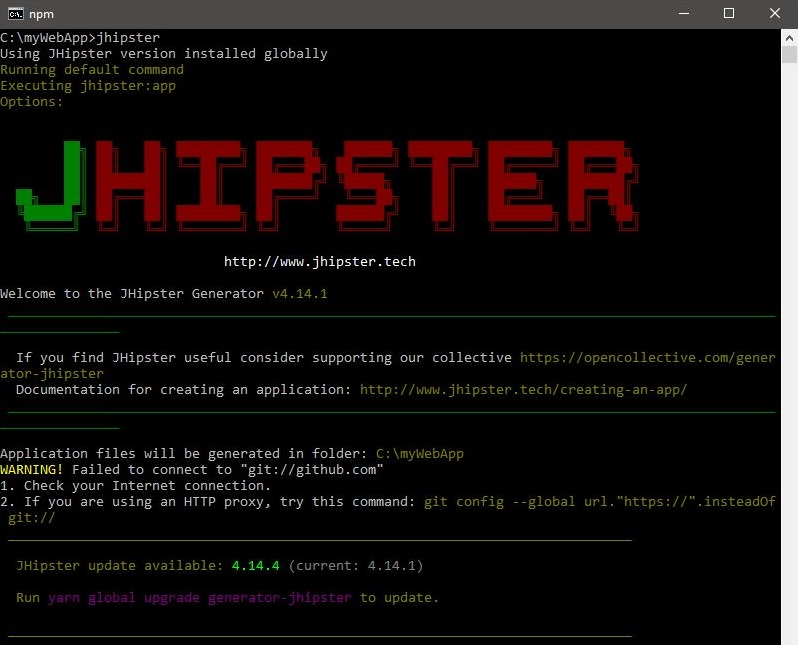
\includegraphics[width=1\textwidth]{2}
\caption{Inicio de JHipster}
\label{fig:2}
\end{center}
\end{figure} 

En este momento será necesario responder a diferentes preguntas para realizar la configuración de la aplicación. La primera pregunta es acerca del tipo de aplicación que se desea generar, en el caso de ONCOSUP, se escogió una aplicación monolítica.

\begin{figure}[!h]
\begin{center}
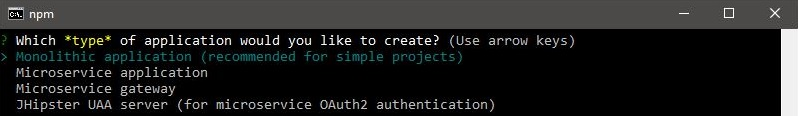
\includegraphics[width=1\textwidth]{3}
\caption{Selección del tipo de aplicación}
\label{fig:3}
\end{center}
\end{figure} 
\clearpage

Tras elegir el tipo de aplicación, se solicitarán la carpeta en la que queremos generarla (la carpeta actual si no se especifica nada) y el paquete por defecto de Java. A la de pregunta de si se desea utilizar \emph{JHipster Registry}, en el caso de ONCOSUP, se responde que no. Respecto al tipo de autenticación JHipster ofrece varias opciones, en este ejemplo se elige HTTM Session Authentication, que es la que usa \emph{Spring Security} por defecto. (Figura \ref{fig:4})

\begin{figure}[!h]
\begin{center}
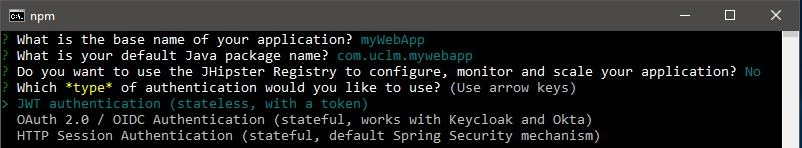
\includegraphics[width=1\textwidth]{4}
\caption{Elección del tipo de autenticación}
\label{fig:4}
\end{center}
\end{figure} 

A continuación, se solicitará información acerca de la base de datos que usará la aplicación (figura \ref{fig:5}). En este caso se elige la primera opción, MySQL, ya que se usará MariaDB, pero hay otras opciones como MongoDB o Cassandra que también pueden seleccionarse.

\begin{figure}[!h]
\begin{center}
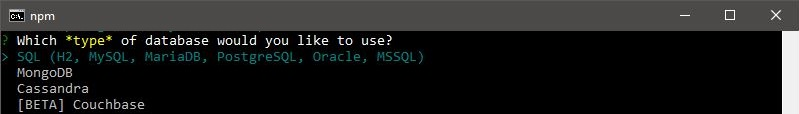
\includegraphics[width=1\textwidth]{5}
\caption{Configuración del tipo de Base de Datos}
\label{fig:5}
\end{center}
\end{figure} 

Se seleccionará MariaDB tanto para producción como para desarrollo. Cuando se pregunte si se quiere usar la abstracción de caché de Spring, se responderá que no, ya que no queremos deshabilitar Hibernate (figura \ref{fig:6}).

\begin{figure}[!h]
\begin{center}
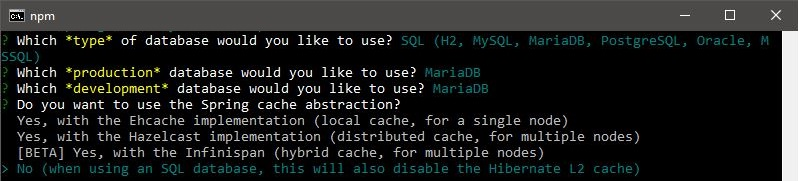
\includegraphics[width=1\textwidth]{6}
\caption{Selección acerca de la abstracción de caché}
\label{fig:6}
\end{center}
\end{figure} 
\clearpage

Para la compilación del proyecto en el back-end se usará Maven y respecto a otras tecnologías se seleccionará el motor de búsqueda con ElasticSeach. Para ONCOSUP no hacía falta ninguna otra tecnología, pero algunas opciones interesantes permiten añadir un login social, para acceder usando cuentas de Google, Facebook o Twitter o añadir un servicio de mensajes asíncronos. Como framework se seleccionará Angular5, aunque hay soporte para todas las versiones de AngularJS.(figura \ref{fig:8})

\begin{figure}[!h]
\begin{center}
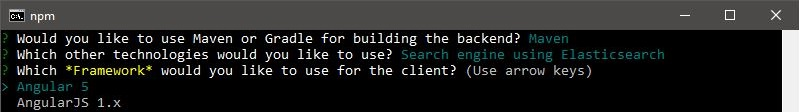
\includegraphics[width=1\textwidth]{8}
\caption{Versiones de Angular a elegir}
\label{fig:8}
\end{center}
\end{figure} 

Se elegirá que no a la pregunta sobre activar soporte para SASS. En cuanto a la internacionalización, en este caso, si queremos tenerla. Como idioma nativo seleccionamos español, y como idiomas adicionales catalán e inglés. La internacionalización permite añadir tantos idiomas como se desee de la lista. (figura \ref{fig:9})

\begin{figure}[!h]
\begin{center}
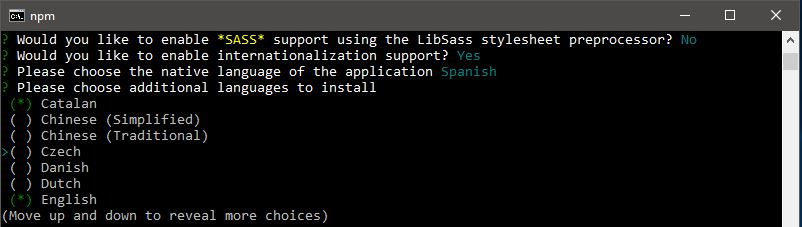
\includegraphics[width=1\textwidth]{9}
\caption{Configuración del idioma principal y secundarios}
\label{fig:9}
\end{center}
\end{figure}

En el caso de este proyecto el presupuesto no permite tener equipo de testing, así no se seleccionará ninguna herramienta adicional de testing. Y por último responderemos que no a instalar otros generadores de la tienda de JHipster. (figura \ref{fig:10})

\begin{figure}[!h]
\begin{center}
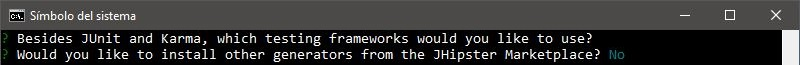
\includegraphics[width=1\textwidth]{10}
\caption{Herramientas de testing disponibles}
\label{fig:10}
\end{center}
\end{figure} 
\clearpage
La figura \ref{fig:11}, a continuación, muestra un resumen de la configuración seleccionada para ONCOSUP.

\begin{figure}[!h]
\begin{center}
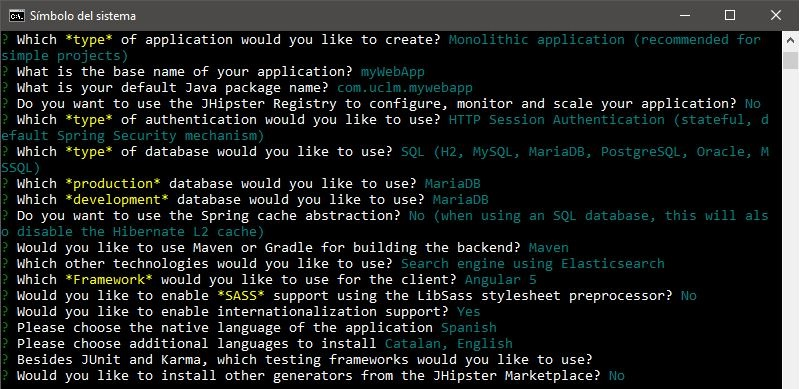
\includegraphics[width=1\textwidth]{11}
\caption{Resumen de la configuración para la aplicación}
\label{fig:11}
\end{center}
\end{figure} 

Con esto, se habrá completado la configuración de la aplicación y se mostrará en pantalla algo similar a lo que se ve a continuación: la instalación de los lenguajes, instalación y resolución de dependencias de paquetes. Finalmente, tras todas las instalaciones que JHipster necesita hacer, mostrará que ha generado de forma exitosa, tanto el cliente como el servidor(figura \ref{fig:14}).

\begin{figure}[!h]
\begin{center}
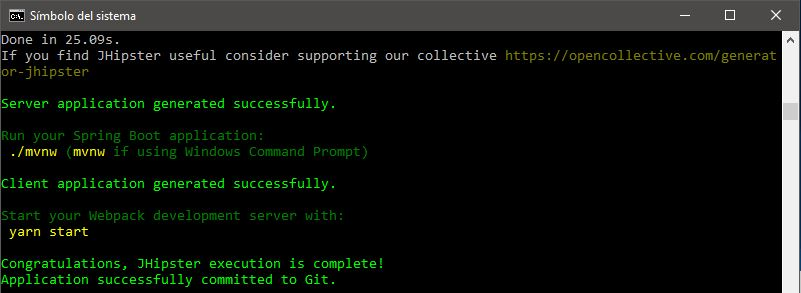
\includegraphics[width=1\textwidth]{14}
\caption{Resultado de la generación}
\label{fig:14}
\end{center}
\end{figure} 

La aplicación ya está generada, pero no hay una estructura de entidades definida, es necesario importar un JDL. En los capítulos \ref{chap:antecedentes} y \ref{chap:resultados}, se trata acerca del JDL, cómo crearlo y algunas de sus características más relevantes. Para este ejemplo se usará un JDL de ejemplo que se puede encontrar en la página de JHipster. La estructura de entidades es la que muestra la figura \ref{fig:JDLejemplo}

\begin{figure}[!h]
\begin{center}
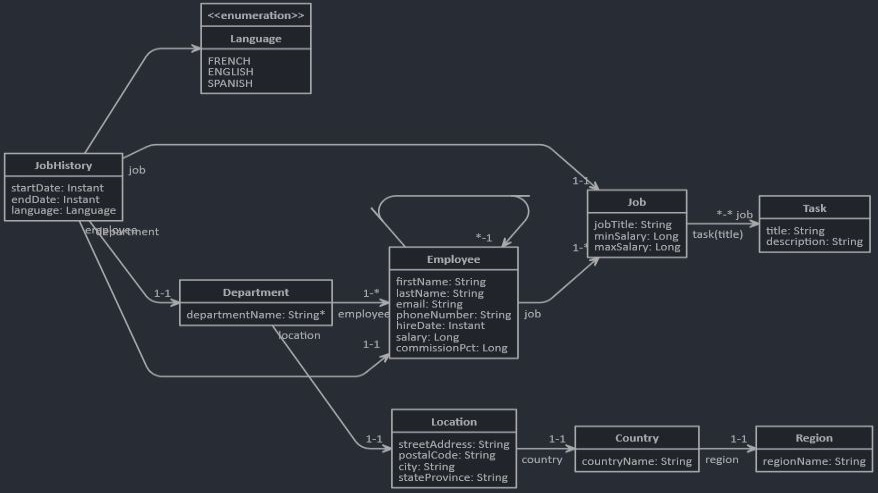
\includegraphics[width=1\textwidth]{JDLejemplo}
\caption{Estructura de entidades usada para la aplicación}
\label{fig:JDLejemplo}
\end{center}
\end{figure}

Tras haber creado nuestro JDL, ya sea en un editor de texto o en la herramienta que proporciona JHipster, JDL-Studio, es necesario importarlo en nuestra aplicación recién generada. Para ello, en la carpeta de nuestro proyecto, donde también hemos dejado nuestro JDL, ejecutamos el comando: \texttt{\$ jhipster import-jdl tuJDL.jh}.

En la consola se irán mostrando las entidades creadas, y en caso de que haya sobrescrituras, como en el caso de los elementos que ya estaban generados, se preguntará si se desea sobrescribir (figura \ref{fig:sobreescribirEntidades}). Para este ejemplo elegimos sobrescribir, pero al realizar modificaciones, es buena opción pensar qué archivos conviene sobrescribir y cuáles no.

\begin{figure}[!h]
\begin{center}
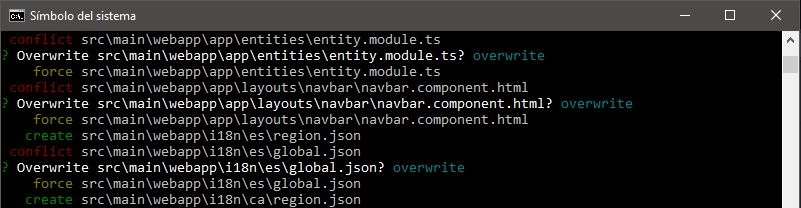
\includegraphics[width=1\textwidth]{sobreescribirEntidades}
\caption{Importación del JDL}
\label{fig:sobreescribirEntidades}
\end{center}
\end{figure}

Una vez se ha respondido a todas las preguntas acerca de sobreescrituras, podremos ver algo similar a lo que muestra la figura \ref{fig:JDLdone}, si todo ha ido correctamente.

\begin{figure}[!h]
\begin{center}
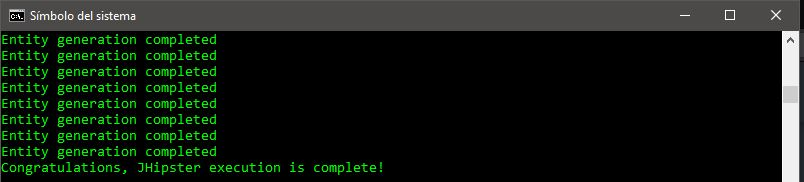
\includegraphics[width=1\textwidth]{JDLdone}
\caption{Resultado de la generación de entidades}
\label{fig:JDLdone}
\end{center}
\end{figure}

La aplicación ya es funcional, se puede compilar y acceder a ella a través del puerto 8080. Para compilar y lanzar la aplicación, tan solo es necesario ejecutar el comando \texttt{\$ mvnw} en la ubicación del proyecto. Si hemos configurado la base de datos podremos autenticarnos y navegar por la aplicación, en caso contrario, tan sólo podremos verla página de inicio (figura \ref{fig:myWebApp}).

\begin{figure}[!h]
\begin{center}
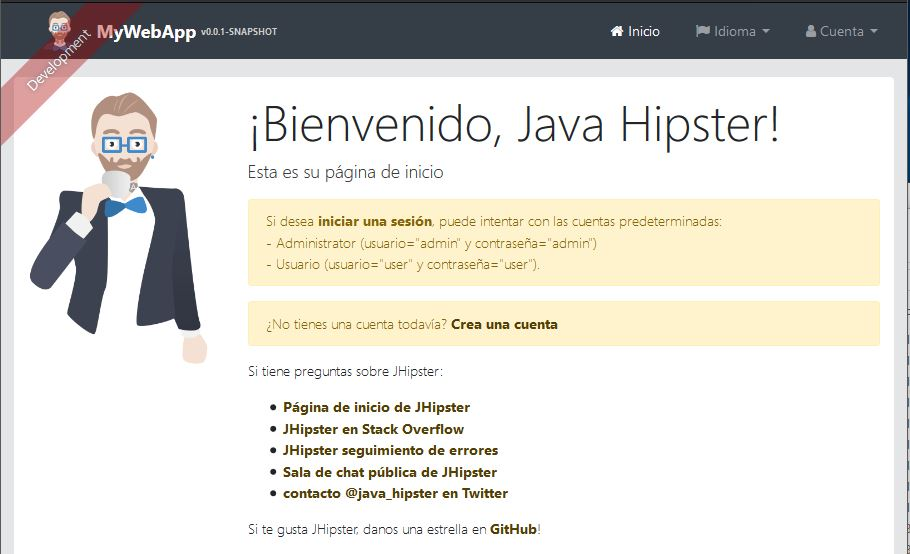
\includegraphics[width=1\textwidth]{myWebApp}
\caption{Página de inicio de la aplicación}
\label{fig:myWebApp}
\end{center}
\end{figure}
